\chapter{The ScienceIE Task: Design and Implementation}

To complete the ScienceIE task, the plan was made to have one Java project containing three sub systems, where each of which could be called independently. As such, this section shall step through each subtask's design and implementation in order, beginning with a description of the preprocessing that was implemented, as it is generic to all subtasks.

After this section has finished describing the design and implenetation of the varous algorithms used in this project, the following section shall describe the results associated with them.

\section{Data Preprocessing}
To support processing in later systems, all data (development, training and test) had to be preprocessed. The idea of this piece of computation is to prepare the data for analysis, and to also reduce computation time (doing this process once for the entire system rather than once for each sub system). To further reduce experiment run time, Java serialisation was also used to save all the following preprocessing information for later retrieval.

In Java, for each paper file from ScienceIE, a \texttt{Paper} object was constructed. This held many important pieces of information about the paper in question, including location on disk, text extracted from its source file, and all preprocessing information. \texttt{Paper} itself is a \textit{plain old Java object}, only holding information and is an abstract class, with \texttt{TextPaper} and \texttt{PDFPaper} classes extending from it which could be instantiated. These extended classes inherited the data storage features and utilities from \texttt{Paper}, but their constructors are customised to extract information from their given type of file:

\begin{itemize}
	\item \texttt{TextPaper} is for \texttt{.txt} files and simply extracts the text from the document. It sees the title of the text document as the title of the paper.
	\item \texttt{PDFPaper} is for \texttt{.pdf} files. This uses Apache PDFBox\footnote{https://pdfbox.apache.org/} (imported through Maven\footnote{https://pdfbox.apache.org/2.0/dependencies.html}) to extract the text from a PDF. The title, once again, is the title of the document. As alluded to earlier, with the ScienceIE test set not only being just text files but also being short documents, longer PDF papers was not usually used, so little development to properly sanitise PDFs happened, meaning all titles and references were also captured in this text extraction. If more PDF files were to be processed this would have been looked at, however, due to its lack of use the time needed to fix this was deemed not worth it.
	\item It was initially planned that there would be a \textit{HTML} and \textit{WebPDF} classes although, for similar reasons to why the \texttt{PDFPaper} text extraction was not developed further, these two classes were never implemented. The main reason for wanting them was to later support the POC system, as this would allow that system to dynamically grab papers from the web and add them to itself. Importing of papers to the POC system shall be discussed later at a more relevant time.
\end{itemize}

The bulk of the preprocessing came in the form of using a parser to calculate the parse tree of a text. As discussed, many teams at ScienceIE used spaCy. As the plan for this project was to complete it in Java (creating a single, self contained system) the Stanford CoreNLP package was used \cite{Manning2014} (imported through Maven\footnote{https://stanfordnlp.github.io/CoreNLP/download.html}). While offering a range of useful NLP features, the main ones utilised by the project were tokenization and finding the parse tree of the text (which naturally included POS tagging). An \texttt{Annotator} class was constructed which accepted a \texttt{Paper} input and annotated the text contained using the CoreNLP library.

Further processing on this information was also completed, where (at the time of saving the CoreNLP parse information) a token \textit{map} was created. This \textit{map}'s key set was all tokens present in the document, with the associated value being the number of times the token was in the document. This was to help when calculating TF-IDF scores later in processing.

The final part of preprocessing was to load existing annotation information. Of course this was only possible for ScienceIE data, which were all supplied with the relevant \texttt{.ann} files in BRAT format. These records were loading into a list of \texttt{Extraction} abstract entities, where each entry to the list could be either of a \textit{KeyPhrase} or \textit{Relationship} extending type, which each held all the information supplied in the annotation files (including classifications, the types of relations and more).

\section{Subtask A - Key Phrase Extraction}
Subtask A at ScienceIE was considered the hardest, reinforced by both the maximum and average scores for each independent subtask. This paper dedicated most of its NLP effort to this task out of the three subtasks as this is currently the hardest part of information extraction (out of the given subtasks) under current research. 

Two attempts at this subtask were made. Initially, a \textit{safer} design involved a SVM which considers some of the key features about key phrases suggested in the literature around this topic. Then, an even more experimental trail shall be described which involves clustering based around Word2Vec similarities between words in a document. 

\subsection{Method 1: Support Vector Machine}
Inspired by the highest success at ScienceIE, a SVM approach was adopted to attempt to provide a solution to subtask A. Initially, a small set of support vectors were selected and tested, with more being added as research continued.

\subsubsection*{Processing Data}
Two approaches were considered when designing the input and output data. One was based around passing each token in individually and in order, while the other was based around using the parse information obtained by using CoreNLP to pass sections of a sentence. 

Working with each individual token was selected for several reasons. Firstly, it was very easy to simply iterate through every token in a document in turn. Furthermore, the CoreNLP data is still available (evidences as that is what returns the tokens of the document) and can be passed to the SVM to be used when calculating support vectors. While using sections of a sentence should help keep any key phrase extracted more semantically correct (i.e. it should avoid missing the end of a noun phrase by accident which a check could be added for anyway), it poses a large issue: Any section selected as a key phrase would likely be \textit{locked down} as such to the specific tokens inside that section, meaning there may be no way to get rid of excess information or added extra if the gold standard key phrase requires something slightly different to the key phrase chosen by the SVM. In terms of extra information needed, a system could be implemented to join adjacent key phrases but that would like see extra information over what is needed being included. If, to try and solve this issue, some system which could extend or retract by a token or two was implemented, it is getting closer to the original option anyway where the system is processing the entire document as individual phrases. Therefore, a system based around processing each token individually was decided upon.

This resulted in a total of 65447 different training points (the total number of individual tokens in all of the training data).

\subsubsection*{Defining Support Vectors}
It is clear that current trends view the position of key phrases are very important in the document and should definitely be considered when trying to learn how to predict them. A tokens proximity to other tokens semantically and as part of the document as whole seem to significantly help us identify where key phrases lie. Furthermore, some attributes about individual phrases also seem to play a large part. For example, the length of the word is a valid feature to evaluate, as the average length of a key phrase token (7 characters) is slightly different to the average of all key phrases (8 characters). 

\begin{table}
	\centering
	\begin{tabular}{ C{7cm} | c }
		\textbf{Support Vector Description} & \textbf{Value Range} \\
		\hline
		The length of the token divided by the maximum token length in the training set. & \texttt{svLen} $\in$ $\mathbb{R}$,  0 $\leq$ \texttt{svLen} $\leq$ 1 \\
		\hline
     	Whether the token is a noun (using Part-Of-Speech tagging). & \texttt{svPos} $\in$ \{0, 1\} \\
     	\hline
     	The TF-IDF score of the token. & \texttt{svTfIdf} $\in$ $\mathbb{R}$,  0 $\leq$ \texttt{svTfIdf} $\leq$ 1 \\
     	\hline
     	The token index divided by the number of tokens. & \texttt{svDepth} $\in$ $\mathbb{R}$,  0 $\leq$ \texttt{svDepth} $\leq$ 1 \\
     	\hline
     	The token index in the current sentence divided by the number of tokens in the sentence. & \texttt{svDepthSentence} $\in$ $\mathbb{R}$,  0 $\leq$ \texttt{svDepthSentence} $\leq$ 1 \\
     	\hline
		Whether the token is in the first sentence of the paper. & \texttt{svFS} $\in$ \{0, 1\} \\
		\hline
     	Whether the token is in the last sentence of the paper. & \texttt{svLS} $\in$ \{0, 1\} \\
     	\hline
     	Whether the previous token was part of a key phrase. & \texttt{svLWKP} $\in$ \{0, 1\} \\
	\end{tabular}
	\caption[Initial Key Phrase Support Vectors]{Initial key phrase support vectors used. A set of these support vectors is generated for each token. When defining the value range, the variable is named as it is in the Java code.}
	\label{table:kpinitsvs}
\end{table}

Thankfully, the idea behind using an SVM is to find what separates key phrases from just normal phrases. Therefore, I was able to create an initial range of support vectors, as defined in table \ref{table:kpinitsvs}. Here it is evident most support vectors are based around trying to gather information as to the whereabouts of the token. It also, importantly, considers the sequence of key tokens.

\subsubsection*{Training}
To train the SVM, a \textit{problem} must be created. The \textit{problem} contains an array of data points, each of which holds a set of support vectors. Each of these data points must be labelled. The label is what we are trying to predict on the test data, so here the label is where or not the token is a key phrase (\texttt{0} for \textit{normal}, or \texttt{1} for key phrase). 

\subsubsection*{Model Selection}
As the nature of the data is unknown, an educated guess can be made as to which kernel to use. A common kernel to begin working with is the \textit{Radial Basis Function} (RBF) kernel \cite{Chih-WeiHsuChih-ChungChang2008}. This is because it can handle non-linear data, which it is assumed the training data here is to be. The RGF kernel function to find the similarity between two data points is listed below:

\begin{equation*}
K\textsubscript{RBF}(x_i, x_j) = exp(-\gamma||x_i - x_j||^2)
\end{equation*}

\noindent There are two parameters which can be configured and tuned to optimise performance of the SVM:
\begin{itemize}
	\item The cost \textit{C} parameter. This influences the misclassification allowance, where a small value lets the SVM select a large hyper-plane for separating data but allows for more misclassification, and a large value will allow the SVM to attempt to find a smaller hyper-plane that has less misclassification. Several values will be explored, of the set \{5, 50, 100, 200\}.
	\item The RBF kernel has a single parameter $\gamma$. From the same source that recommended the RBF kernel, as a initial value the SVM shall be configured to 0.5, as this is 1 divided by the number of features (we have 2 labels). However, other values shall be explored to attempt to find the best accuracy, and these values shall be \{0.25, 0.5, 1\}.
\end{itemize}

\subsubsection*{Development}
Having decided on how to use the concept of an SVM, there was a need for a concrete implementation. The idea of implementing an SVM was considered, however, with a responsibly high implementation complexity and a high risk of getting something subtly wrong (therefore being hard to detect and fix) a pre-existing solution was searched for. Furthermore, with the author having never handled an SVM before, a pre-existing solution with additional usage information was desired.

A popular SVM package was found in libsvm (imported through Maven\footnote{https://mvnrepository.com/artifact/com.datumbox/libsvm/3.22}). Originally written in C and ported over to Java (as well as many other languages), libsvm was designed to be flexible, supporting various kernels and suitable for beginners through to advanced users. It has support for the core use of SVMs - training and predicting, but also has features to aid in parameter selection such as a cross-validation function (which will be covered in more detail shortly), a visualiser for the training data and a data scaling tool.

% TODO add more about development

\subsubsection*{Cross Validation}
Cross validation is an important part when trying to optimise performance of an SVM. It allows for tuning key parameters by running repeated tests. Rather than using the testing data, which could introduce bias, the training data is split up into \textit{n} folds (or groups of data from within the training set). \textit{n = 5} folds were used in this instance. In turn, the SVM is trained with 4 of the 5 folds and then evaluated against the remaining fold. This is repeated for all combinations of folds and then the accuracy of the SVM can be calculated. A higher accuracy should mean better performance, although there is the problem of over fitting to consider. If the model is built to run perfectly on the training data, real world performance may actually suffer. This is why we cannot stop testing the SVM after just cross validation, as evaluating against the unseen test set will tell us how well it really performs. 

\begin{center}
	\begin{figure}
		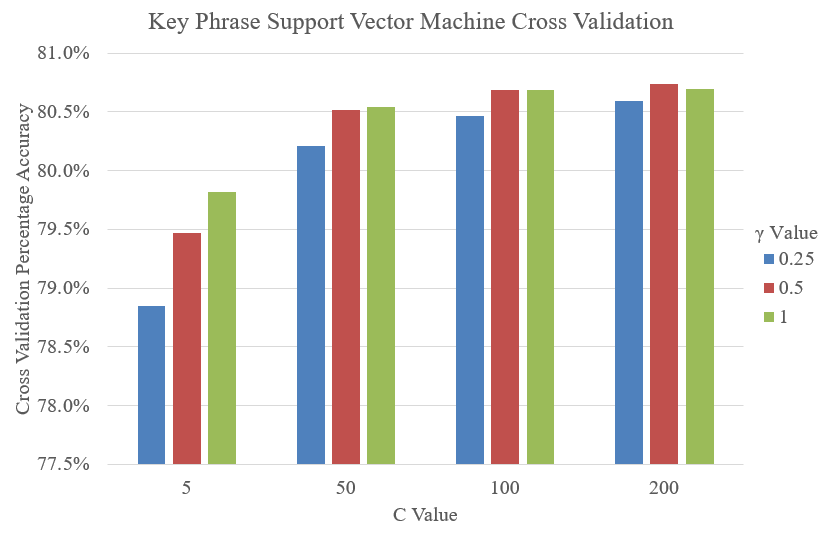
\includegraphics[width=\textwidth]{img/kpsvmcrossvalidation.png}
		\caption[Key Phrase SVM Cross Validation]{The cross validation results on the key phrase SVM.}
		\label{figure:kpsvmcv}
	\end{figure}
\end{center}

The values discussed for \textit{C} and $\gamma$ were used in cross validation and their outputs compared. The cross validation results can be seen in figure \ref{figure:kpsvmcv}. As show by this chart, very little change is accuracy is observed. There is a upward trend as \textit{C} and $\gamma$ increase, but this appears to plateau as higher values are evaluated. No smaller values need testing as (given the trend continues) the accuracy will significantly diminish. In terms of increasing the values, there is potential for extremely small gains; however, the return from increasing these values will be almost worthless and the training time required as the \textit{C} value increase significantly rises, as the SVM is working harder to find a better fitting hyper plane. Therefore, \text{C = 100} and \textit{$\gamma$ = 0.5} shall be used when completing full experiments. While, a \textit{C} value of 200 is 0.05\% more accurate with the same $\gamma$ value, the training time is roughly doubled (from some hours to many hours) and the reward is not deemed worth it.

\subsection{Method 2: Clustering}
\subsubsection*{Concept}
Clustering has been shown to be effective in key phrase and other information extraction. A seemingly effective method was using \textit{term relatedness} to group terms, and then find an exemplar term at the centre of the clusters which can be used as a key phrase \cite{Liu2009}. 

Inspired by this, this paper proposes a similar process, where the similarity of terms is based around their Word2Vec similarities. Conceptually, it is possible that gathering similar terms will have the effect of creating clusters of important concepts, from which key phrases can be extracted. With the most similar words at the centre, these could be considered key words, and the phrase around these words could be extracted from the document. This should also exclude unimportant or stop words, as these may have large distances to the key concepts. 

An important note here is that the document is treated as a \textit{bag-of-words}, where we ignore the semantic meaning of the words. Word2Vec does this anyway, as when using the library the word is simply passed as plain text with no extra information, and Word2Vec uses its own ideas about the words semantic meanings to evaluate it. Using a bag-of-words approach means words from any part of the document could be clustered together, which is ok as if both are close to the centre of a cluster, it may mean both of them are key phrase worthy and should be selected (a full phrase from their origin extracted to be a key phrase).

The clustering algorithm selected was hierarchical clustering \cite{Rai2010}. Bottom up (agglomerative) hierarchical clustering works as follows:
\begin{enumerate}
	\item Each element begins in their own cluster (so \textit{n} elements means initially there are \textit{n} clusters).
	\item Given some distance metric, the distances between all clusters are calculated.
	\item The closest two clusters are combined.
	\item This process is repeated until a single cluster is left.
\end{enumerate}
\noindent This algorithm was chosen for several reasons:
\begin{itemize}
	\item Firstly, it is a relatively straight forward clustering algorithm to implement, so should allow results to be found quickly.
	\item While the term similarities are based off of Word2Vec similarities, the distances between clusters could be evaluated in a number of ways. These include \textit{single} (the shortest distance between terms in each cluster), \textit{average} (the average distance between each term in one cluster to each term in another) and \textit{complete} (the largest distance between terms n each cluster). These are called the \textit{linkage criteria}.
	\item If successful, the benefits of using clustering could be two fold. Not only might this produce effective key phrases, but it may even aid in classification. Once a number of clusters have formed key phrases, the hierarchical clustering could continue potentially all the way to producing just a few clusters where each could be classified into one of our 3 target classes. This will only be successful if the key phrase extraction is successful. If doing this clustering was purely for classification, k-means clustering may be more appropriate with a \textit{k = 3} where each cluster would be a different classification.
\end{itemize}

When working with hierarchical clustering, an important aspect to consider is how far to iterate through the algorithm. In theory, the algorithm should run until there is just one cluster left with every element in it - but this is not useful for anything. The more useful cluster states will be part of the way along the iterative cycle. To find this \textit{sweet spot} will require manual tuning, via inspecting the progression of the clusters to try to identify a good range where key phrase information can be extracted. In theory finding the sweet spot could be automated and learnt (by trying to extract key phrases at all levels and evaluating against the gold standard phrases to see how well the algorithm does) but to fully develop this kind of system would require a lot of time, which itself is very expensive, and if a failure it would be a big waste of time.

A large difference between this and SVM usage is that this method is unsupervised learning and does not require training data, while using an SVM is supervised learning. This means that, given this method works for this testing scenario, its application may scale better in the \textit{real world} as is it not tied to the quality of the training data. Furthermore, given a suitable Word2Vec model, differences in key phrase output may be seen. This means that this algorithm may suffer here given the Word2Vec models currently available are not based on scientific publications, but running this algorithm on test data with similar context to the Word2Vec model may improve things, which means it may even cope with different languages.

\subsubsection*{Development}
The process of turning this theory into a practical implementation is straight forward. To allow for future expansion if clustering was to be used again for anything, a generic abstract \texttt{Cluster} class was created, which was formed of a list (where type is specified at creation time) of items and declaration of functions to find the distance between a given cluster object and another cluster, and to create a new cluster by combining a given cluster object with another.

A \texttt{Linkage} enumeration was created which could be used when testing to specify the method for finding the distance between two clusters.

Actually commencing the clustering begins by splitting the document into all of its tokens, and removing duplicates. Then, stop words and unimportant words are removed. Unimportant words are classified based on their TF-IDF scores. All words were sorted according to their TF-IDF score, and the bottom 15\% were removed. This percentage was manually set, after generating a list of all tokens and their TF-IDF scores and evaluating where the cut off should be to remove all words that are not in any key phrase and that are not very interesting words. Some care needed to be taken, as for example, "results" has a low TF-IDF score of 0.006, but is in the key phrase "generalization of these results to the NSI case". Of course, that phrase also includes other words like "of", "the" and "to" which would be removed, but when we have some key words we could then reintroduce the semantic information and try to form well formed snippets, and as "results" would connect the first and second half of the sentence to help form the full phrase it is important to not get rid of all unimportant words. Therefore, 15\% was found to be a reasonable compromise to remove the particularly low TF-IDF valued tokens and to leave the rest of the some what to very interesting tokens in the bag-of-words.

Then, the process of hierarchical clustering happens as described above. This happens for all test data, with all three linkage methods, with results being saved to disk. The output is then evaluated on a sample of the processed documents (as manually reviewing all 100 test documents cluster patterns across 3 different linkage criteria is too much for a single reviewer to achieve) to try to evaluate where key phrases can be extracted from.

\section{Subtask B - Key Phrase Classification: Word2Vec}
With a large amount of influence coming from Word2Vec, the decision was made to focus on exploiting this technology to try to classify key phrases.

As the whole concept of Word2Vec is word similarities based on their semantic meaning, the idea is proposed that simply examining the distance from a key phrase to the relevant classification term or similar may result in a reasonably accurate classification. 

An important thing to consider is that Word2Vec generally accepts individual tokens. This contrasts to what we are trying to classify which is a string of tokens. Therefore, a way to find the similarity between a string of tokens and a singular token must be devised.

Two methods for achieving a distance metric are proposed and shall be tested:
\begin{itemize}
	\item Average distance: each token in the string of tokens are compared to the target token and their distances are averaged,
	\item Shortest distance: each token in the string of tokens are compared to the target token the shortest distance (highest value in terms of \textit{similarity}) is used.
\end{itemize}

There is also the problem of token importance - as it is like not all tokens will aid in classifying a key phrase. For example, "determine the lowest energy configuration" has the word "the" as a token. This token is bad as it can be used in a key phrase with any classification, and likely not make any difference. Therefore, it is theorised that stop words and very low TF-IDF words being removed could help improve classification results. There is a potential downside to this, as some key phrases may appear as only containing stop words. "He" for example is a key phrase and is a synonym of "helium", but without that relation knowledge (which at this stage of the competition we in theory doesn't have) it would be seen as a stop word and removed. In this case it would actually nullify the key phrase so should be left and classification attempted anyway, but this is why this algorithm should be tested with and without unimportant words being removed, as not all of them may actually be unimportant.

\begin{table}
	\centering
	\begin{tabular}{ c | c }
		\textbf{Target Class} & \textbf{Similar Word Set to use when Testing} \\
		\hline
		Task & Task, Application, Goal, Problem \\
		 \hline
		Process & Process, Model, Algorithm\\
		 \hline
		Material & Material, resource \\
	\end{tabular}
	\caption[Word2Vec Classification Target Words]{The target classes and the set of words that are of a similar domain to be used in testing of the Word2Vec classifier.}
	\label{table:w2vclasswords}
\end{table}

Finally, there is the question of what token to find similarity too. A simple way forward is comparing the tokens to the word identifying the class we're trying to find out about, so simply testing for similarity to "test", "process" and "material". However, if the quality of the Word2Vec model isn't very good (it could have an incorrect idea about what a \textit{task} is) the classification may be of poor quality as well. To try to solve this problem, more words based around the same concept should be tested against to try to avoid the problem of a single word being in the incorrect space in Word2Vec vector space. Therefore, when testing this algorithm the similarities will be based on the word of the defining class ("task", "process", "material") on one set of runs, and on the other set of runs the maximum similarity to words related to that of the class shall be found. The words that shall be used are defined in table \ref{table:w2vclasswords}. The original word for the class shall still be evaluated when finding the maximum similarity from a set of similar words.

\section{Subtask C - Relation Extraction: Support Vector Machine}
A section all about what I did for part 3
\subsection{Many Support Vectors}
Discuss the SVM I tried to do this with (including Word2Vec)
\subsection{Few Support Vectors}

